% Propósito: distinguir una conformación espectral de referencia de una banda
% estrecha y mostrar qué parámetros deben especificarse en cada caso.
% Origen: definiciones de las secciones \ref{sec:u10-ruido-vocal} y
% \ref{sec:u10-nbn}; B=f_H-f_L, ecuación \eqref{eq:u10-ancho-nbn}.
% Curvas y bloques cualitativos; no representan una norma ni un equipo.
% Descripción accesible: dos cadenas parten de ruido de banda ancha. La cadena
% superior atraviesa un filtro cuya respuesta H_v(f) posee una magnitud
% objetivo especificada y produce ruido con forma espectral vocal. La inferior
% atraviesa un filtro pasa banda de respuesta H_B(f), delimitado por f_L y
% f_H, centrado en f_c, y produce NBN.
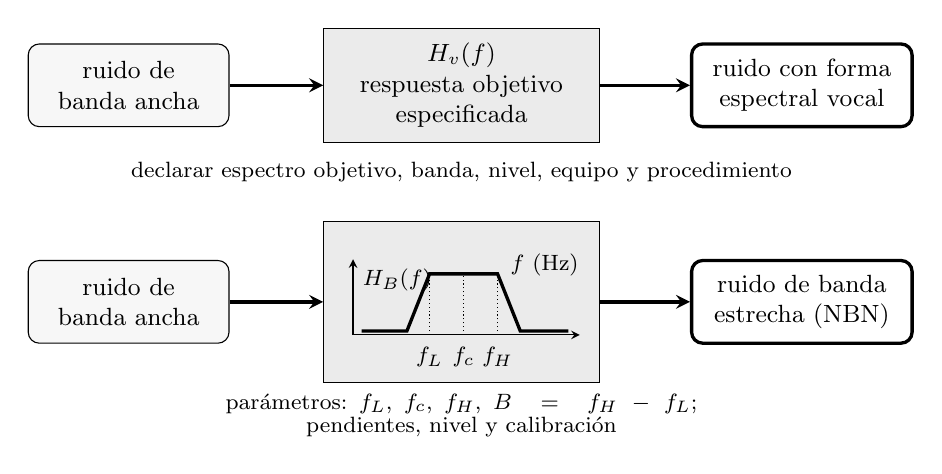
\begin{tikzpicture}[
    x=0.95cm,
    y=1cm,
    >=stealth,
    font=\small,
    bloque/.style={
        draw,
        rounded corners,
        minimum width=2.55cm,
        minimum height=1.05cm,
        align=center,
        fill=black!3
    },
    filtro/.style={
        draw,
        minimum width=3.50cm,
        minimum height=1.45cm,
        align=center,
        fill=black!8
    },
    salida/.style={
        draw,
        rounded corners,
        minimum width=2.80cm,
        minimum height=1.05cm,
        align=center,
        very thick
    }
]
    \node[bloque] (entrada-v) at (1.55,4.65)
        {ruido de\\banda ancha};
    \node[filtro] (filtro-v) at (6.00,4.65)
        {\(\lvert H_v(f)\rvert\)\\
         respuesta objetivo\\especificada};
    \node[salida] (salida-v) at (10.55,4.65)
        {ruido con forma\\espectral vocal};
    \draw[->,very thick] (entrada-v) -- (filtro-v);
    \draw[->,very thick] (filtro-v) -- (salida-v);

    \node[align=center,font=\footnotesize,text width=8.4cm]
        at (6.00,3.55)
        {declarar espectro objetivo, banda, nivel, equipo y procedimiento};

    \node[bloque] (entrada-b) at (1.55,1.90)
        {ruido de\\banda ancha};
    \node[filtro,minimum height=2.05cm] (filtro-b) at (6.00,1.90) {};
    \node[salida] (salida-b) at (10.55,1.90)
        {ruido de banda\\estrecha (NBN)};
    \draw[->,very thick] (entrada-b) -- (filtro-b);
    \draw[->,very thick] (filtro-b) -- (salida-b);

    \begin{scope}[shift={(4.55,1.48)},x=0.72cm,y=0.62cm]
        \draw[->] (0,0) -- (4.00,0);
        \node[font=\footnotesize] at (3.38,1.43)
            {\(f\) (Hz)};
        \draw[->] (0,0) -- (0,1.55);
        \node[below right,font=\footnotesize] at (0,1.55)
            {\(\lvert H_B(f)\rvert\)};
        \draw[very thick]
            (0.15,0.08) -- (0.95,0.08) -- (1.35,1.25) --
            (2.55,1.25) -- (2.95,0.08) -- (3.80,0.08);
        \draw[densely dotted] (1.35,0) -- (1.35,1.25);
        \draw[densely dotted] (1.95,0) -- (1.95,1.25);
        \draw[densely dotted] (2.55,0) -- (2.55,1.25);
        \node[below=1pt,font=\footnotesize] at (1.35,0) {\(f_L\)};
        \node[below=1pt,font=\footnotesize] at (1.95,0) {\(f_c\)};
        \node[below=1pt,font=\footnotesize] at (2.55,0) {\(f_H\)};
    \end{scope}

    \node[align=center,font=\footnotesize,text width=10.0cm]
        at (6.00,0.46)
        {parámetros: \(f_L,\ f_c,\ f_H,\ B=f_H-f_L\);\\[-1pt]
         pendientes, nivel y calibración};
\end{tikzpicture}
